\section{函数列与函数项级数}
\label{sec:ru-function-sequences}

前几节的极限对象都是数。很多时候，我们用一系列函数逐步逼近同一个对象：几何级数的部分和$1+x+\cdots+x^N$逼近$1/(1-x)$，指数级数的部分和逼近$e^x$。
这时每个编号$n$对应一整个函数$f_n:X\to\mathbb R$，$(f_n)$称为\term{函数列}（sequence of functions）。
固定编号，看到的是一个函数；固定输入$x$，看到的是一列数$(f_n(x))_{n\geq1}$。函数列的收敛可以从后一个角度出发，但我们还关心收敛对整个函数意味着什么。

函数项级数$\sum_kg_k$的部分和$S_N=\sum_{k\leq N}g_k$本身就是一个函数列，级数的收敛与和函数都由部分和的极限决定。
所以下文先对函数列建立结论，再把它们用于部分和，不另建一套收敛语言。

\subsection{逐点收敛与一致收敛}
\label{sec:ru-pointwise-uniform}

最直接的做法是在每个输入处分别取数列极限。若对每个$x\in X$，数列$(f_n(x))$都收敛到$f(x)$，称$f_n$在$X$上\term{逐点收敛}（pointwise convergence）到$f$。
按数列极限的定义，这是说：对每个$x$和每个$\varepsilon>0$，存在$N$使$n\geq N$时$|f_n(x)-f(x)|<\varepsilon$，其中$N$可以随$x$改变。
若要求一个尾部起点同时控制全部输入，就得到更强的条件。
\begin{definition}[一致收敛]
\label{def:ru-uniform-convergence}
若对每个$\varepsilon>0$，都存在$N$，使$n\geq N$时对\emph{所有}$x\in X$都有$|f_n(x)-f(x)|<\varepsilon$，称$f_n$在$X$上\term{一致收敛}（uniform convergence）到$f$。
\end{definition}
两种收敛的差别与连续和一致连续的差别相同，都在于量词次序：$N$是否允许随$x$改变。

$f_n(x)=x^n$在$[0,1]$上的行为说明了这种差别。$0\leq x<1$时$x^n\to0$，$x=1$时恒为$1$，所以$f_n$逐点收敛到函数$f$，$f$在$[0,1)$上为$0$、在$1$处为$1$。
但在$x$接近$1$的地方，要使$x^n<1/2$，需要$n>\log2/\log(1/x)$，这个下界在$x\to1^-$时无界，没有一个$N$能同时管住所有$x$。
图~\ref{fig:ru-power-sequence-nonuniform}画出了几条$x^n$：无论$n$多大，曲线在靠近$1$处都要从接近$0$升到$1$，最大误差始终不小。

\begin{figure}[!htbp]
 \centering
 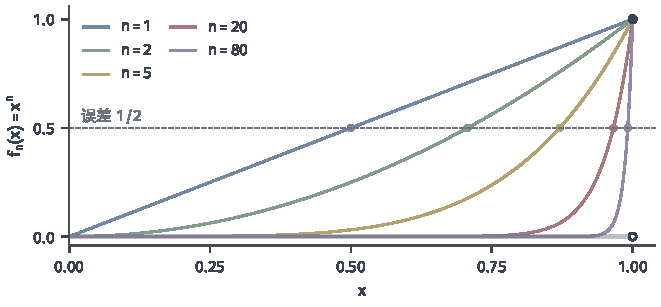
\includegraphics[width=112mm]{figures/01-mathematical-preliminaries-upper/02-real-numbers-and-univariate-functions/matplotlib/power-sequence-nonuniform/figure.pdf}
 \caption{函数列$f_n(x)=x^n$在$[0,1]$上的几条曲线（$n=1,2,5,20,80$）。逐点极限在$[0,1)$上为$0$（灰色水平线），在$x=1$处为$1$（实心点）。虚线标出误差$1/2$：每条曲线都在$x=2^{-1/n}$处越过它，越过位置随$n$增大逼近$1$，所以$\sup_{[0,1)}|f_n-f|=1$，收敛不一致。图为解析示例。}
 \label{fig:ru-power-sequence-nonuniform}
\end{figure}

\paragraph{一致收敛的判别}
直接检查一致收敛的办法是看最大误差。记$\|f_n-f\|_\infty=\sup_{x\in X}|f_n(x)-f(x)|$，则$f_n$一致收敛到$f$，当且仅当这个数列趋于零：两者说的都是“误差界可以对全部输入同时缩小”。
对$x^n$，在$[0,1)$上$\sup|x^n-0|=1$，不趋于零，所以收敛不一致；但在$[0,\rho]$（$\rho<1$）上，最大误差为$\rho^n\to0$，收敛是一致的。
可见一致收敛也依赖定义域，问题只出在$x=1$附近。这里的$\sup$只是一列数值的上确界，我们并没有把函数当作某个空间中的点。

不知道极限函数时，也可以用柯西条件检验。
\begin{theorem}[一致柯西准则]
\label{thm:ru-uniform-cauchy}
函数列$(f_n)$在$X$上一致收敛到某个函数，当且仅当对每个$\varepsilon>0$，存在$N$，使$m,n\geq N$时对所有$x\in X$都有$|f_m(x)-f_n(x)|<\varepsilon$。
\end{theorem}
\begin{proof}
必要性由三角不等式得到。对充分性，每个固定的$x$处$(f_n(x))$是柯西数列，因此收敛，记极限为$f(x)$。
在$|f_m(x)-f_n(x)|<\varepsilon$中固定$n\geq N$与$x$，令$m\to\infty$，得到$|f(x)-f_n(x)|\leq\varepsilon$，这个界对所有$x$同时成立。
\end{proof}

把一致柯西准则用于部分和，得到函数项级数最常用的判别法：用一列可求和的数值上界控制各项。
\begin{theorem}[Weierstrass判别法]
\label{thm:ru-weierstrass-m-test}
若存在非负数$M_k$，使$|g_k(x)|\leq M_k$对所有$x\in X$和$k$成立，且$\sum M_k<\infty$，则$\sum_kg_k$在$X$上一致收敛，并且对每个$x$绝对收敛。
\end{theorem}
\begin{proof}
对$m>n$，$|S_m(x)-S_n(x)|\leq\sum_{k=n+1}^m|g_k(x)|\leq\sum_{k>n}M_k$，右侧与$x$无关且随$n$增大趋于零，由一致柯西准则即得一致收敛；每个$x$处的绝对收敛由比较判别得到。
\end{proof}
例如$\sum_k\sin(kx)/k^2$在$\mathbb R$上一致收敛，可取$M_k=1/k^2$。第~\ref{sec:ru-power-series}节将用这一判别法证明幂级数在内部闭子区间上一致收敛。

\subsection{函数列连续性的保持}
\label{sec:ru-uniform-limit-continuity}

$x^n$的例子中，每个$f_n$都连续，逐点极限却在$1$处跳跃。所以逐点收敛不能保持连续性。一致收敛补上了缺失的一步。
\begin{theorem}[一致极限保持连续]
\label{thm:ru-uniform-limit-continuity}
若每个$f_n$在$a\in X$处连续，且$f_n$在$X$上一致收敛到$f$，则$f$在$a$处连续。特别地，连续函数列的一致极限是连续函数。
\end{theorem}
\begin{proof}
给定$\varepsilon>0$，由一致收敛选$n$使$|f_n(x)-f(x)|<\varepsilon/3$对所有$x$成立；再由$f_n$在$a$处连续选$\delta$，使$|x-a|<\delta$时$|f_n(x)-f_n(a)|<\varepsilon/3$。于是
\[
 |f(x)-f(a)|\leq|f(x)-f_n(x)|+|f_n(x)-f_n(a)|+|f_n(a)-f(a)|<\varepsilon.
\]
\end{proof}
证明把总误差拆成三段：两次用$f_n$逼近$f$的误差，以及固定函数$f_n$自身的连续误差。关键在于第一段和第三段用的是同一个$n$，并且这个$n$对点$x$和点$a$同时有效。
逐点收敛时，能让$|f_n(x)-f(x)|$变小的$n$可能随$x$改变，$x$越靠近$a$，所需的$n$越大，三段误差就无法同时控制；$x^n$在$1$附近正是这种情况。

把定理用于部分和：若每个$g_k$连续，且$\sum g_k$在$X$上一致收敛，则和函数连续，因为部分和是有限个连续函数之和。
结合Weierstrass判别法，$\sum\sin(kx)/k^2$的和函数在$\mathbb R$上连续。至于求导、积分能否与这种极限交换，分别留到第~\ref{sec:ru-termwise-differentiation}节与第~\ref{sec:ru-termwise-integration}节。
